\documentclass[9pt]{amsart}
\usepackage[paperheight=8.4in,paperwidth=6in,margin=0.5in]{geometry}
%\geometry{landscape}                % Activate for for rotated page geometry
%\usepackage[parfill]{parskip}    % Activate to begin paragraphs with an empty line rather than an indent
\usepackage{graphicx}
\usepackage{amssymb}
\usepackage[framemethod=tikz]{mdframed}
\usepackage{tcolorbox}
\usepackage{xstring,xifthen} % string length with conditionals
\usepackage{epstopdf}
\DeclareGraphicsRule{.tif}{png}{.png}{`convert #1 `dirname #1`/`basename #1 .tif`.png}

% LUKE'S SETTINGS
% packages
\usepackage{framed}
\usepackage{xcolor}
\usepackage{hanging}
% paragraph
\setlength\parindent{0pt}
\setlength{\parskip}{1em}
% margins
%\addtolength{\oddsidemargin}{0.25in}
\addtolength{\topmargin}{-0.15in}
\addtolength{\textheight}{0.7in}
% colored border with mdframed
\definecolor{agred}{RGB}{151, 54, 41}
\definecolor{agskin}{RGB}{243, 211, 189}
\definecolor{ltgray}{RGB}{250, 250, 250}
\definecolor{lighttan}{HTML}{FBEEAC}
\definecolor{pale}{HTML}{FFF9D0}
\newmdenv[innerlinewidth=1.5pt, roundcorner=4pt, linecolor=agred, innerleftmargin=6pt,
innerrightmargin=6pt, innertopmargin=6pt, innerbottommargin=6pt, backgroundcolor=pale]{myboxA}
% colored border with tcolorbox
\newtcbox{\myboxB}{nobeforeafter,colframe=bordercolor,colback=bordercolor!10!white,boxrule=0.5pt,arc=4pt,
  boxsep=0pt,left=6pt,right=6pt,top=6pt,bottom=6pt,tcbox raise base}
% frame
\definecolor{shadecolor}{rgb}{0.95,0.95,0.95}
% fixed width font (Courier)
\renewcommand{\ttdefault}{pcr}
% san-serif font (Helvetica)
\usepackage[scaled]{helvet}
\renewcommand\familydefault{\sfdefault} 
\usepackage[T1]{fontenc}
% column widths with any alignment
\usepackage{array}
\newcolumntype{L}[1]{>{\raggedright\let\newline\\\arraybackslash\hspace{0pt}}m{#1}} % left-mid
\newcolumntype{C}[1]{>{\centering\let\newline\\\arraybackslash\hspace{0pt}}m{#1}}   % center-mid
\newcolumntype{R}[1]{>{\raggedleft\let\newline\\\arraybackslash\hspace{0pt}}m{#1}}  % right-mid
\newcolumntype{X}[1]{%
 >{\vbox to 2ex\bgroup\vfill}%
 p{#1}%
 <{\egroup}} 
 
% no extra space after period
\frenchspacing

% Macros file generated by trading_cards_2_macros_figures.ipynb
\def\sequence{TACGGAAGGTCCGGGCGTTATCCGGATTTATTGGGTTTAAAGGGAGCGTA
GGCCGTCTGTTAAGCGTGTTGTGAAATGTCGGGGCTCAACCTGGGCATTG
CAGCGCGAACTGGCAGACTTGAGTG}
\def\taxonomyGG{k\_\_Bacteria; p\_\_Bacteroidetes; c\_\_Bacteroidia; o\_\_Bacteroidales; f\_\_Prevotellaceae; g\_\_Prevotella; s\_\_stercorea}
\def\wikipedia{Prevotella is a genus of Gram-negative bacteria.
Prevotella spp. are members of the oral and vaginal flora, and are recovered from anaerobic infections of the respiratory tract. These infections include aspiration pneumonia, lung abscess, pulmonary empyema, and chronic otitis media and sinusitis.}
\def\prevalencePercent{1.34}
\def\prevalenceRank{971}
\def\abundancePercent{0.0223}
\def\abundanceRank{424}
\def\numOTUs{27248}
\def\trimLength{125}
\def\numSamples{9511}
\def\rarefactionDepth{1250}


% No page numbers
\thispagestyle{empty}

% Document
\begin{document}

%\begin{framed} % alt: shaded

\begin{myboxA}

\begin{center}

\includegraphics[width=12cm]{../agp_header.pdf}
\end{center}

\hspace{1.07cm}
\begin{tabular}{L{5in}}
\texttt{\sequence{}}
\end{tabular}

\noindent
\begin{minipage}[t]{.48\textwidth}
\raggedright
\begin{hangparas}{1em}{1}
    TAXONOMY:   \taxonomyGG{}
\\ \vspace{2mm}
    WIKIPEDIA:  \wikipedia{}
\end{hangparas}
\end{minipage}%
\hfill
\begin{minipage}[t]{.48\textwidth}
\raggedright
\begin{hangparas}{1em}{1}
    PREVALENCE: Found in \prevalencePercent{}\% of 9,511 samples, %\numSamples{}
                rank \#\prevalenceRank{} out of 27,248 sequences. %\numOTUs{}
\\ \vspace{2mm}
    ABUNDANCE:  Composes \abundancePercent{}\% of 11.9M observations,
                rank \#\abundanceRank{} out of 27,248 sequences. %\numOTUs{}
\\ \vspace{2mm}
    METHODS:    Amplicon PCR with 16S rRNA V4 primers 515f--806rB.
    			Sequenced with Illumina MiSeq (150~bp).
                Error-corrected with Deblur, trimmed to \trimLength{}~bp, and
                rarefied to 1,250 observations per sample. %\rarefactionDepth{}
                Showing 9,511 samples from the American Gut cohort. %\numSamples{}
\end{hangparas}
\end{minipage}

RELATIVE DISTRIBUTION BY METADATA:

\begin{raggedright}
\begin{tabular}{C{6cm} C{6cm}}
Age & Types of plants per week\\
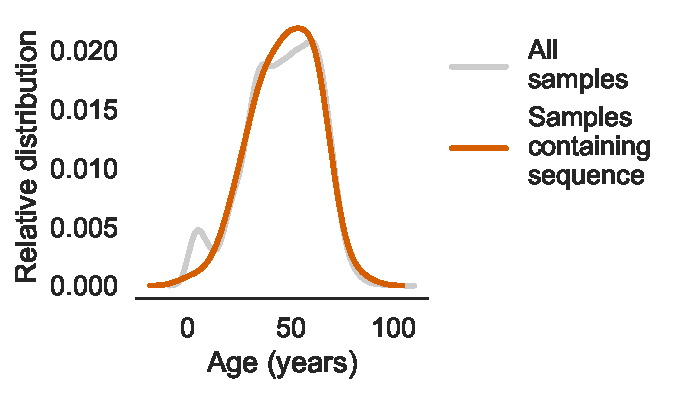
\includegraphics[height=3.6cm]{kde_age_years.pdf} & 
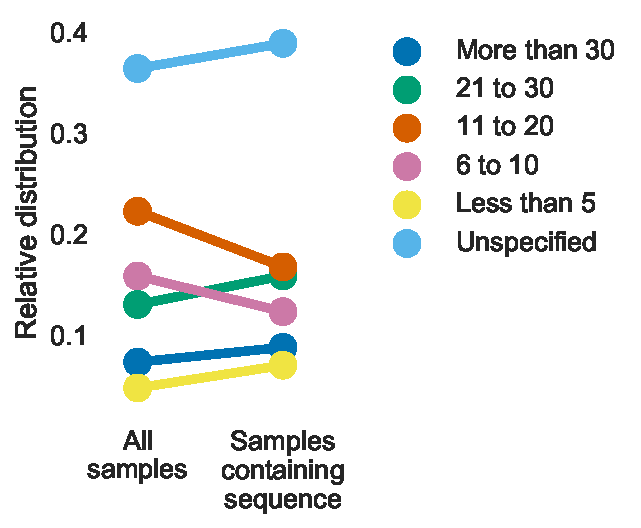
\includegraphics[height=4.6cm]{point_types_of_plants.pdf}\\ \\
\end{tabular}
\end{raggedright}

\vspace{-1cm}

SEARCH TRENDS:

\begin{raggedright}
\begin{tabular}{C{12cm}}
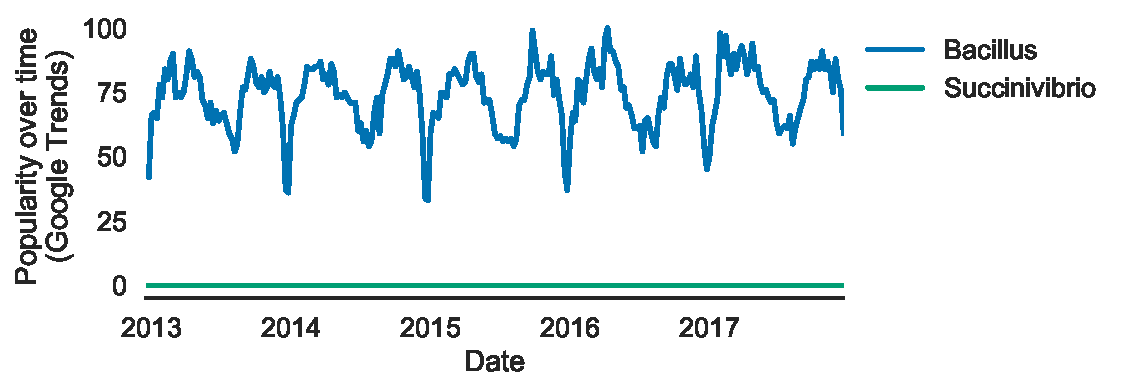
\includegraphics[height=3.6cm]{trends.pdf}
\end{tabular}
\end{raggedright}

%\begin{raggedright}
%\begin{tabular}{C{6cm} C{6cm}}
%Age & Longitude\\
%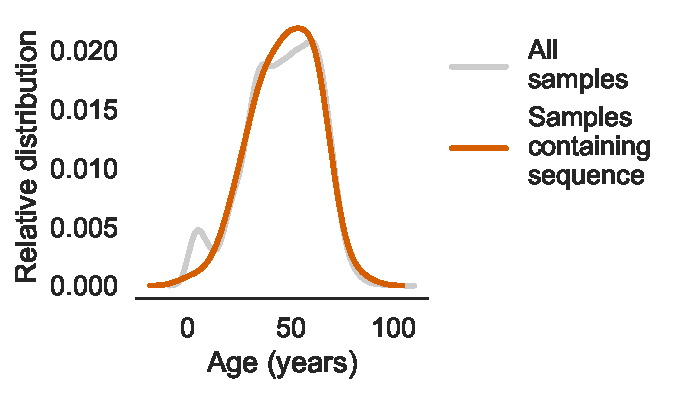
\includegraphics[height=3.2cm]{kde_age_years.pdf} & 
%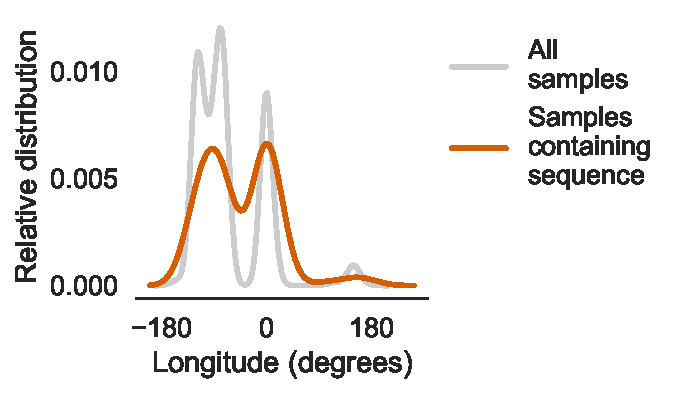
\includegraphics[height=3.2cm]{kde_longitude.pdf}\\ \\
%Last usage of antibiotics & Types of plants per week\\
%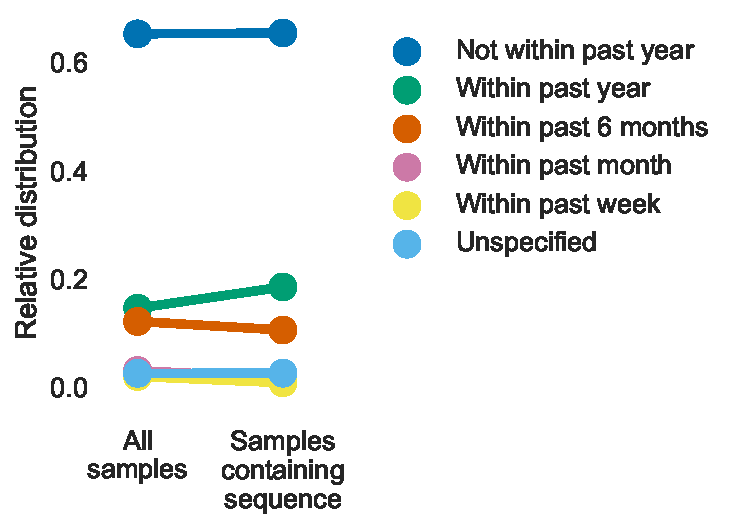
\includegraphics[height=4.4cm]{point_antibiotic_history.pdf} & 
%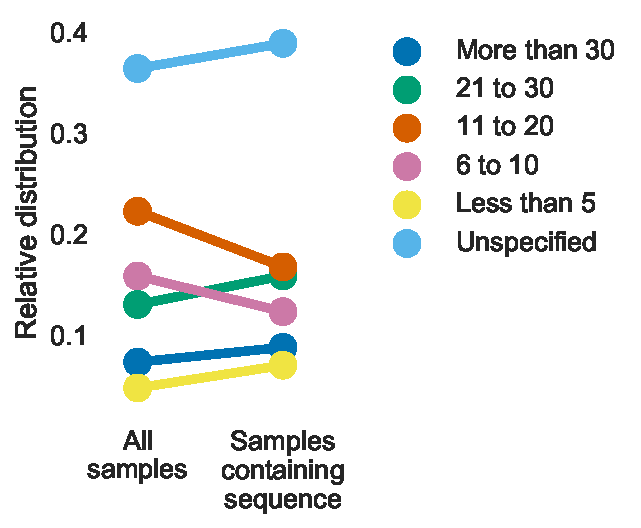
\includegraphics[height=4.4cm]{point_types_of_plants.pdf}\\
%Fruit frequency & Prepared meals frequency\\
%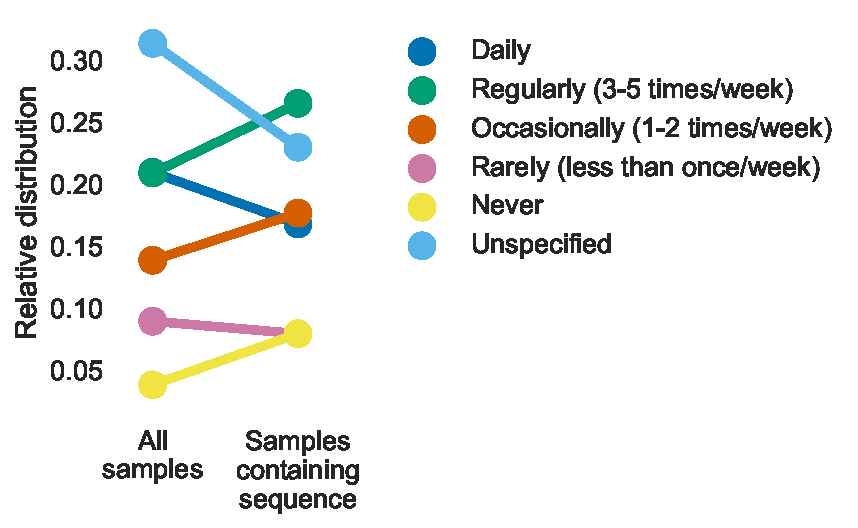
\includegraphics[height=4.4cm]{point_fruit_frequency.pdf} &
%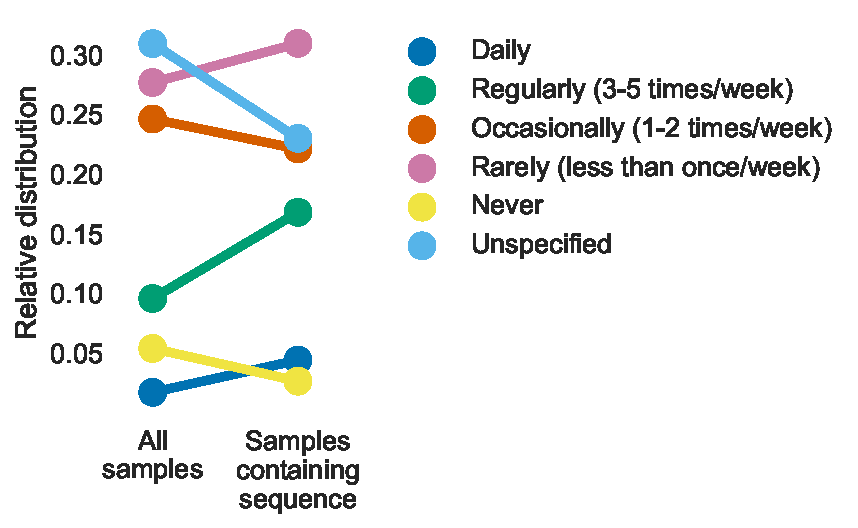
\includegraphics[height=4.4cm]{point_prepared_meals_frequency.pdf}\\ 
%\end{tabular}
%\end{raggedright}

%\begin{center}
%	\copyright{} 2017 American Gut Project
%\end{center}

\end{myboxA}

%\end{framed}


\end{document}  
